% !TeX root = RJwrapper.tex
\title{Pomdp: A Computational Infrastructure for Partially Observable Markov Decision Processes}
\author{by Michael Hahsler and Anthony R. Cassandra}

\maketitle

\abstract{%
Many important problems involve decision-making under uncertainty. For example, a medical professional needs to make decisions about the best treatment option based on limited information about the current state of the patient and uncertainty about outcomes. Different approaches have been developed by the applied mathematics, operations research, and artificial intelligence communities to address this difficult class of decision-making problems. This paper presents the \CRANpkg{pomdp} package, which provides a computational infrastructure for an approach called the partially observable Markov decision process (POMDP), which models the problem as a discrete-time stochastic control process. The package lets the user specify POMDPs using familiar R syntax, apply state-of-the-art POMDP solvers, and then take full advantage of R's range of capabilities, including statistical analysis, simulation, and visualization, to work with the resulting models.
}

\hypertarget{introduction}{%
\section{Introduction}\label{introduction}}

Many important problems require decision-making without perfect information,
and where decisions made today will affect the future.
For example, in diabetes prevention and care, the primary care
provider needs to make decisions about screening, early interventions
like suggesting lifestyle modification, and eventually
medication for disease management
based on a patient's available medical history. Especially,
screening and lifestyle modifications need to be used early on to
be effective in preventing severe and debilitating diseases later on.
This is clearly a difficult problem that involves uncertainty and
requires a long-term view. We have studied this problem
using the partially observable Markov decision process approach in
(Kamalzadeh et al. 2021) and, in the absence of solvers for R,
we started the development of the \texttt{pomdp}
package described in this paper.

A Markov decision process (MDP)
is a discrete-time stochastic control process that models
how an agent decides on what actions to take when facing an environment
whose dynamics can be adequately modeled by a Markov process that can be
affected by the agent's behavior (Puterman 1994).
That is, the environment transitions between a set of states
where transition probabilities only depend on the current state and
are conditioned on the agent's actions.
Over time, the agent receives rewards depending on the actions and the
environment's state. The agent's objective is to make a plan that
maximizes its total reward earned.
A plan can be expressed as a mapping of each possible state
to the best action in that state.
The best possible plan is often called the optimal policy.
For MDP problems, the agent is always aware of
the state of the environment and can make decisions directly following such a policy.

A partially observable Markov decision process (POMDP) generalizes the
concept of the MDP to model more realistic situations where the agent
cannot directly observe the environment's state.
Here, the agent must
infer the current state using observations that are only probabilistically linked to
the underlying state. The agent can form a belief about what states
it may be in and update its belief when new observations are made.
In this setting, the agent has to base its actions on its current belief.
A POMDP can be modeled as a \emph{belief MDP} where the underlying Markov model uses belief states instead of the original states of the environment.
While the original state space is typically modeled as a finite set of states, making MDPs readily solvable using dynamic programming, the agent's belief is represented by a probability distribution over the states in the form of a continuous probability simplex
and are therefore much more challenging to solve.
The volume of the believe space that POMDPs are operating in grows
exponentially with the number of underlying states.
This is called the curse of dimensionality which means that working with
problems with a
realistic number of states typically requires the use of approximate algorithms.

Karl Johan Åström first described Markov decision processes with
a discrete state space and imperfect information in 1965
(Åström 1965). The model was also studied by the operations research community where the acronym POMDP was introduced (Smallwood and Sondik 1973).
More recently, the POMDP framework was adapted for automated planning problems in artificial intelligence (Kaelbling, Littman, and Cassandra 1998).
The POMDP framework is a popular choice when a known Markov process can adequately approximate system
dynamics and the reward function is known. POMDPs have been successfully applied to
model various real-world sequential decision processes.
Examples include numerous industrial, scientific, business, medical and military applications where an optimal or near-optimal policy is needed. This includes important applications like machine maintenance scheduling, computer vision, medical diagnosis, and many more. A detailed review of applications can be found in (Cassandra 1998a).

While the (PO)MDP framework is used to find an optimal or near optimal policy, given
a model of system dynamics, the related class of model-free reinforcement learning algorithms, more specifically, temporal difference learning, Q-learning and its deep learning variations (Sutton and Barto 2018),
learn unknown system dynamics and
the reward function directly from interactions with the environment.
Reinforcement learning methods typically require observable states and perform a large amount of exploration, where the agent performs sub-optimal actions to learn about the environment.
Q-learning and some algorithms are already available in R packages like \CRANpkg{ReinforcementLearning} (Proellochs and Feuerriegel 2020).
While these model-free approaches are very powerful for many artificial intelligence applications, they may not be appropriate
for situations where experts already possess a reasonable
amount of knowledge about the system dynamics and where
the cost of sub-optimal actions is very high. For example, the cost of administering the wrong medication in a medical setting
due to exploration by a pure reinforcement learning approach may not be acceptable and a model-based approach like a POMDP is more appropriate.
The R package described in this paper exclusively focuses on planning with POMDP.

While POMDPs are well studied, the complexity of solving all but very small problems
limits its application.
Recent spectacular advances in artificial intelligence applications have lead to more interest in POMDPs, as
shown in the development of new approximate algorithms and
by the frameworks available for various programming languages:

\begin{itemize}
\tightlist
\item
  pomdp-solve (Cassandra 2015) is a C program to solve POMDPs using exact and approximate solvers.
\item
  APPL (APPL Team 2022) provides the fast point-based POMDP solver SARSOP in C++.
\item
  ZMDP software (Smith 2009) implements several approximate value iteration algorithms in C++.
\item
  pyPOMDP (Migge and Stollmann 2013) is a Python 2.x toolbox for solving POMDPs.
\item
  JuliaPOMDP (JuliaPOMDP Team 2022) is a set of packages for defining and solving MDPs and POMDPs using the Julia programming language.
\end{itemize}

R activity around POMDPs has also picked up with the packages \CRANpkg{sarsop} (Boettiger, Ooms, and Memarzadeh 2021) and \CRANpkg{pomdpSolve} (Hahsler and Cassandra 2022) which interface the
two popular POMDP solver programs APPL and pomdp-solver.

In this paper, we present \CRANpkg{pomdp} (Hahsler 2023) which was co-developed with
\CRANpkg{pomdpSolve} (Hahsler and Cassandra 2022) to provide R users with
a consistent and flexible infrastructure for solving and working with
POMDPs. The package can be used to work with larger POMDP problems but is limited
by the capability of the used solvers. Larger problems also typically lead to
very complicated policies which can be executed by an automatic agent but
are not very helpful for a human user. This paper
focuses on features for smaller problems that yield simpler policies. Such models and
policies are better suited for human experts who want to understand the problem and
are interested in improved decision making.
For example, a medical researcher who tries to
develop easy-to-follow guidelines for doctors based on experiments with a POMDP model
is looking for a relatively simple and robust model with a simple and
understandable policy.
This typically means
to consider a model with few states and a small number of different observations.
For example, we have used the package to study diabetes
prevention by creating a very small, simplified model
to obtain a policy that is actionable in a primary care setting (Kamalzadeh et al. 2021).
A second use of smaller models is in a classroom or self-study setting where the \CRANpkg{pomdp}
package can be used to demonstrate and study how POMDP models, solvers, and resulting
policies work.

\hypertarget{background-for-partially-observable-markov-decision-processes}{%
\section{Background for partially observable Markov decision processes}\label{background-for-partially-observable-markov-decision-processes}}

A POMDP is a discrete-time stochastic control process that can formally be described by the 7-tuple
\[\mathcal{P} = (S, A, T, R, \Omega , O, \gamma),\] where

\begin{itemize}
\tightlist
\item
  \(S = \{s_1, s_2, \dots, s_n\}\) is the set of partially observable states of the environment,
\item
  \(A = \{a_1, a_2, \dots, a_m\}\) is the set of available actions,
\item
  \(T\) describes the system dynamics as the set of transition probabilities \(T(s' \mid s,a)\)
  the state transition \(s \rightarrow s'\) conditioned on taking
  ion \(a\).
\item
  \(R: S \times A \times S \rightarrow \mathbb{R}\) is the reward function which can
  depend on the\\
  the state transition (previous and new state) and the action,
\item
  \(\Omega = \{o_1, o_2, \dots, o_k\}\) is the set of possible observations,
\item
  \(O\) defines the probabilistic connection of observations with the reached states \(s'\) as the set of observation probabilities \(O(o \mid a, s')\) conditioned on the action \(a\) taken to reach \(s'\), and
\item
  \(\gamma \in [0, 1]\) is the discount factor modeling how much the agent prefers immediate rewards over later rewards.
\end{itemize}

The used notation follows largely (Kaelbling, Littman, and Cassandra 1998). Several variations of
this notation can be found in the literature.
Sets are often set in calligraphic font and it is also common to see the
observation model denoted by \(Z\) instead of \(O\).

The control process proceeds in discrete time steps called epochs as follows.
At each time epoch \(t\), the environment is in some
unknown state \(s \in S\).
The agent chooses an action \(a \in A\), which causes the environment to
transition to state \(s' \in S\) with probability \(T(s' \mid s,a)\). Simultaneously, the agent receives an observation \(o \in \Omega\), which
depends on the action and the new state of the environment following
the conditional probability distribution \(O(o \mid a, s')\). Finally, the agent receives a reward \(R(s,a,s')\) depending on the transition. This
process repeats till a specified time horizon is reached. Often,
as in the equation below, an infinite horizon
is used.
The goal of the agent is to plan a policy that prescribes actions that
maximize the expected sum of discounted future rewards, i.e., she
chooses at each time \(t\) the action that maximizes

\[\mathbb{E}\left[\sum_{t=0}^{\infty} \gamma^t r_t\right],\]

where \(r_t = R(s_t, a_t, s_{t+1})\) is the reward at epoch \(t\) which depends on the state transition and the action at that time.
Since state transitions are stochastic,
the expectation is taken over all trajectories that the process may take.
Infinite horizon problems are guaranteed to converge if the discount factor \(\gamma < 1\).
For a finite time horizon, the expectation is calculated over the sum up to the end of the
time horizon and a discounted expected final reward (called terminal value) may be added in the final epoch.

In a POMDP, the agent does not know the state the system is in, but it has to use
observations
to form a belief of what states the system could be in. This belief is called a belief state \(b \in B\) and is
represented in the form of a probability distribution over the states. \(B\) is the infinite set of all possible belief states
forming a \(|S|-1\) simplex.
The agent starts with an initial belief \(b_0\) (often a uniform distribution) and then updates the belief when new
observations are available.
In each epoch, after observing \(o\), the
agent can perform a simple Bayesian update where the
updated belief for being in state \(s'\) written as \(b'(s')\) is

\[
b'(s') = \eta\ O(o | a, s') \sum_{s \in S} T(s' | s,a) b(s),
\]
and

\[
\eta = \frac{1}{\sum_{s' \in S}\left( O(o | a, s') \sum_{s \in S} T(s' | s,a) b(s)\right)}
\]
normalizes the new belief state so all probabilities add up to one.

Regular MDPs have (under some assumptions) a deterministic optimal policy that prescribes an optimal action for
each state (Puterman 1994). Even though
the actual states are not observable for POMDPs, POMDPs also have a
deterministic optimal policy that prescribes an optimal action for
each belief state.
A policy is a mapping \(\pi: B \rightarrow A\) that prescribes
for each belief state an action.
The optimal policy is given by

\[\pi^* = \mathrm{argmax}_\pi \  V^\pi(b_0)\]

with

\[V^\pi(b_0) =   \mathbb{E}\left[\sum_{t=0}^{\infty} \gamma^t r_t  \ \bigg\vert \ \pi, b_0 \right].\]

\(V^\pi(b_0)\)
is called the value function given policy \(\pi\) and the agent's
initial belief \(b_0 \in B\). The value function for any MDP or POMDP is a piecewise linear function that can be described by the
highest-reward segments of
a set of intersecting hyperplanes. The parameters for these hyperplanes are typically called \(\alpha\)-vectors and
are a compact way to specify
both, the value function and the policy of the solution of a problem.

For the infinite-horizon case, the policy converges for \(\gamma < 1\)
to a policy that is independent of the time step and the initial belief. In this case, the policy can be visualized as
a directed graph called the policy graph. Each node of the graph is related to a hyperplane and represents the part of the belief space
where this hyperplane produces the highest reward in the
value function. Each node is labeled with the action to be taken given by the policy.
The outgoing edges are labeled with observations and specify to what segment of the value function the agent will transition
given the previous segment, the action and the observation.
The formulation can be easily extended to the finite-horizon case. However, the finite-horizon policy depends on the initial belief and the epoch. The finite-horizon policy forms a policy tree, where each level represents an epoch.

It has to be mentioned that finding optimal policies for POMDPs is known to be
a prohibitively difficult problem because the belief space grows exponentially with the number of states.
This issue is called the \emph{curse of dimensionality} in dynamic programming.
Mundenk (Mundhenk 2000) has shown that finding the optimal policy for POMDPs is, in general, an
\(\text{NP}^\text{PP}\)-complete problem which means that it is at least as difficult as the hardest
problems in \(\text{NP}\).
Therefore, exact algorithms can be only used for extremely small problems that are typically
of very limited use in practice.
More useful algorithms fall into the classes of approximate value iteration and approximate policy iteration (Cassandra 1998b; Hauskrecht 2000), which often find good solutions for larger problems.
However, to use POMDPs successfully,
the researcher typically needs to experiment with simplifying the problem description
and choosing an acceptable level of approximation by the algorithm.

The solution of POMDPs can be used to guide the agent's actions. Automatic agents can follow very complicated
policies. Humans often prefer simpler policies, even if they are not optimal but good enough
to robustly improve outcomes. Simpler policies also result from problem simplification and allowing for a larger degree of approximation by the solver algorithm.

\hypertarget{implementation}{%
\section{Implementation}\label{implementation}}

Package \CRANpkg{pomdp} includes a convenient and consistent way for users to define all components of a POMDP
model using familiar R syntax, solve the problem using several methods and then analyze and visualize the results.
An important design decision is to separate the tasks of defining a problem and analyzing the policy from
the actual solver.
The separation between the infrastructure in
package \CRANpkg{pomdp} and the
solver code makes sure that additional solvers can be easily added in the future.
Solver code is typically interfaced by writing a standard problem definition file, running an external process,
and reading the results back. This way of interfacing solvers has several advantages:

\begin{itemize}
\tightlist
\item
  Using an external process, rather than directly interfacing the code in R ensures that memory issues for larger problems do not compromise the running R process itself.
\item
  The separation lets the solver use any available parallelization technique without imposing limitations
  by R.
\item
  Most existing solver software accepts a standard problem definition file format.
\item
  The problem definition and the results are typically very small and fast to write and read compared to the significant amount of time used by the solver.
\item
  Separating problem definition and result analysis from the actual solver lets the user solve larger problems
  on a dedicated server.
\end{itemize}

For communication with the solver, the package supports the widely used POMDP (Cassandra 2015) file specification and can use POMDPX files (APPL Team 2022) via package \CRANpkg{sarsop}. This means that
new algorithms that use these formats can be easily interfaced in the future, and that
problems already formulated in these formats can be directly solved using the package.
The authors also provide an initial set of solvers with the companion package \CRANpkg{pomdpSolve} which
provides an easy-to-install distribution of the well-known fast C implementation of a set of solvers originally developed by one of the co-authors (Cassandra 2015).
The package \CRANpkg{pomdp} currently provides access to the following algorithms:

\begin{itemize}
\tightlist
\item
  Exact value iteration

  \begin{itemize}
  \tightlist
  \item
    Enumeration algorithm (Sondik 1971; Monahan 1982).
  \item
    Two pass algorithm (Sondik 1971).
  \item
    Witness algorithm (Littman, Cassandra, and Kaelbling 1995).
  \item
    Incremental pruning algorithm (Zhang and Liu 1996; Cassandra, Littman, and Zhang 1997).
  \end{itemize}
\item
  Approximate value iteration

  \begin{itemize}
  \tightlist
  \item
    Finite grid algorithm (Cassandra 2015), a variation of point-based value iteration to solve larger POMDPs (PBVI; see (Pineau, Gordon, and Thrun 2003)) without dynamic belief set expansion.
  \item
    SARSOP (Kurniawati, Hsu, and Lee 2008), Successive Approximations of the
    Reachable Space under Optimal Policies, a point-based algorithm
    that approximates optimally reachable belief spaces for
    infinite-horizon problems (via the third-party
    R package \CRANpkg{sarsop} (Boettiger, Ooms, and Memarzadeh 2021)).
  \end{itemize}
\end{itemize}

While exact methods can only solve very small problems, PBVI and
SARSOP can efficiently find approximate solutions for larger
problems with thousands of states and hundreds of different
observations. \CRANpkg{pomdp} uses by default the finite grid
algorithm.

The \CRANpkg{pomdp} package provides efficient support by using

\begin{itemize}
\tightlist
\item
  sparse matrix representation based on the \CRANpkg{Matrix} package (Bates, Maechler, and Jagan 2022) for large transition and observation
  matrices of low density,
\item
  fast matrix operations,
\item
  fast C++ implementations of loops using \CRANpkg{Rcpp} (Eddelbuettel 2013), and
\item
  parallel execution using \CRANpkg{foreach} (Microsoft and Weston 2022).
\end{itemize}

The package implements many auxiliary functions to analyze and visualize POMDPs and their solution.
For example, to sample from the belief space, simulate trajectories through a
POMDP and estimate beliefs, fast C++ implementations (using \CRANpkg{Rcpp} (Eddelbuettel 2013)) and
support for parallel execution using \CRANpkg{foreach} (Microsoft and Weston 2022) are provided.
To represent and visualize policy graphs the widely used and powerful \CRANpkg{igraph} package (Csardi and Nepusz 2006)
with its advanced layout options is used. Interactive policy graphs can be produced based on the
\CRANpkg{visNetwork} (Almende B.V. and Contributors and Thieurmel 2022).
While the package does not directly provide functions to create \CRANpkg{ggplot2} visualizations (Wickham 2016) to
avoid installing the large number of packages needed, the manual pages provide examples.

Solving a new POMDP problem with the \CRANpkg{pomdp} package consists of the following steps:

\begin{enumerate}
\def\labelenumi{\arabic{enumi}.}
\tightlist
\item
  Define a POMDP problem using the creator function \texttt{POMDP()} using R syntax,
\item
  solve the problem using \texttt{solve\_POMDP()} which calls an external solver, and
\item
  analyze and visualize the results with functions like \texttt{plot\_policy\_graph()}, \texttt{plot\_value\_function()}, and \texttt{reward()}.
\end{enumerate}

We will now discuss these steps in more detail and then present the complete code for a small toy example.

\hypertarget{defining-a-pomdp-problem}{%
\subsection{Defining a POMDP problem}\label{defining-a-pomdp-problem}}

The \texttt{POMDP()} creator function has as its arguments the
7-tuple \((S, A, T, R, \Omega , O, \gamma)\),
the time horizon with terminal values, the
initial belief state \(b_0\) and a name for the model. Default values are an infinite time
horizon (which has no terminal values), and an initial belief state given by a uniform distribution over all states.

While specifying most parts of the POMDP is straightforward, some arguments can be specified for convenience in
several different ways. Transition probabilities,
observation probabilities
and the reward function
can be
specified in several ways:

\begin{itemize}
\item
  A named list of dense or sparse matrices or the keywords \texttt{"identity"} and \texttt{"uniform"} representing the
  probabilities or rewards organized by action.
\item
  As a \texttt{data.frame} representing a table with states, actions and the probabilities or reward values created with the helper functions

  \begin{itemize}
  \tightlist
  \item
    \texttt{T\_(action,\ start.state,\ end.state,\ probability)},
  \item
    \texttt{O\_(action,\ end.state,\ observation,\ probability)} and
  \item
    \texttt{R\_(action,\ start.state,\ end.state,\ observation,\ value)}.
  \end{itemize}

  \texttt{NA} is used to mean that a value applies to all actions, states or observations.
\item
  An R function with the same arguments as \texttt{T\_()}, \texttt{O\_()} or \texttt{R\_()} that
  returns the probability or reward.
\end{itemize}

More details can be found in the manual page for the constructor function \texttt{POMDP()}.

\hypertarget{accessing-model-data}{%
\subsection{Accessing Model Data}\label{accessing-model-data}}

Several parts of the POMDP description can be defined in different ways. In particular, transition probabilities, observation
probabilities, rewards, and the start belief can be defined using dense matrices, sparse matrices, data frames, functions, keywords or a mixture of all of these. The decision to specify different parts of the description using different formats is
typically a result of how it is easier for the user to specify the part of the model.
\# and memory considerations.
For example, transition and observation matrices can typically be represented efficiently as sparse matrices and the keywords \texttt{uniform} and \texttt{identity}, while rewards are typically more compactly specified as a data frame with rows describing the reward for
a subset of action/state/observation combinations.

To write code that performs computation using this information requires a way to access the data in a unified
way. The package provides accessor functions like:

\begin{itemize}
\item
  \texttt{start\_vector()} translates the initial probability vector description into a numeric vector.
\item
  Transition probabilities, observation probabilities, and rewards can be accessed using functions ending in \texttt{\_matrix()}.
  Given an action, a matrix is returned.
  The user can request a dense or sparse matrix using the logical parameter \texttt{sparse}.
  To reduce the overhead associated with representing dense matrices in sparse format, sparse matrices are only returned
  if the density of the matrix is below 50\%. The user can also specify \texttt{sparse\ =\ NULL},
  which will return the data in the way it was specified by the user (e.g., a data frame). This saves the cost of conversion.
  Functions ending in \texttt{\_val()} can be used to access individual values directly.
\end{itemize}

To allow a user-implemented algorithm direct access to the data in a uniform way, \texttt{normalize\_POMDP()} can be used to create a
new POMDP definition where transition probabilities, observation probabilities, rewards, and the start belief are
consistently translated to (lists of) matrices and numeric vectors. Similar access
facilities for C++ developers are also available in the package source code.

\hypertarget{solving-a-pomdp}{%
\subsection{Solving a POMDP}\label{solving-a-pomdp}}

POMDP problems are solved with the function \texttt{solve\_POMDP()}. This function uses the low-level interface in the companion package
\CRANpkg{pomdpSolve} to solve a pomdp using the pomdp-solve software and return a solved instance of the POMDP problem.
Since the low-level interfaces vary between solvers, pomdp will provide additional functions for other popular solvers.
For example, for using the SARSOP solver interfaced in package \CRANpkg{sarsop}, a function \texttt{solve\_SARSOP()} is provided.

Solving POMDPs is often done by trial-and-error while simplifying the problem description to make it
tractable. This means that we need to be able to interrupt the solver when it is running too long or
when it runs out of memory. To accomplish this, the problem is transferred to the solver
by writing a POMDP or POMDPX file, the solver software is then run in a separate process, and the results are read back. This approach results in a more robust interface since the R process is not compromised by a solver that runs out of memory or is interrupted due to too long run time. However, note that writing a large problem description file
can be quite slow.

The \texttt{solve\_POMDP()} and \texttt{solve\_SARSOP()} functions require a POMDP model and then
allow the user to specify or overwrite model parameters that are often used in experimentation
like the horizon, the discount rate, and the initial belief state. Additionally, solver-specific parameters
like the used algorithm for pomdp-solve can also be specified.

\hypertarget{analyzing-the-solution}{%
\subsection{Analyzing the solution}\label{analyzing-the-solution}}

The function \texttt{solve\_POMDP()} returns a solved instance of the POMDP as a list that contains the original
problem definition and an additional element
containing the solution including if the solution has converged, the total expected reward given the initial belief, and the \(\alpha\)-vectors representing the value function \(V^\pi\) and the policy \(\pi\).
Keeping the problem definition and the solution together allows the user to
resolve an already solved problem multiple times experimenting with different initial beliefs, horizons or
discount rates,
and also to perform
analysis that requires both the problem definition and the solution.

An example of such an analysis is to simulate trajectories for a solved POMDP by following
an \(\epsilon\)-greedy policy.
An \(\epsilon\)-greedy policy follows the policy given in the solution but with a probability of \(\epsilon\) uses a random action instead,
which can lead to exploring parts of the belief space that would not be reached by using only the policy.
Such a simulation needs access to the policy in the solution but also to the original problem description
(transaction and observation probabilities). This simulation is implemented in function \texttt{simulate\_POMDP()}
and includes fast C++ code using \CRANpkg{Rcpp} (Eddelbuettel 2013) and a native R implementation supporting
sparse matrix representation and sparse matrix operations.
Both implementations support parallelization using \CRANpkg{foreach} (Microsoft and Weston 2022)
to speed up the simulation.

Often it is also interesting to test the robustness
of a policy on slightly modified problem descriptions or to test
the performance of a manually created policy. These experiments are supported
using function \texttt{add\_policy()} which provides a convenient way to combine POMDP problem descriptions with compatible policies.

While the list elements of the solution can be directly accessed, several convenient access and visualization functions are provided.
We provide a \texttt{plot\_value\_function()} that visualizes the piecewise linear value function giving the reward over the belief space simplex as a line chart for two-state problems. Function \texttt{plot\_belief\_space()}
provides a more flexible visualization of the reward, the policy-based action, or the policy graph node
over the whole belief space. A three-state problem has a belief space of the form of a 2-simplex which is a triangle
and the visualization uses a ternary plot.
The belief space from more than three states cannot be directly visualized, however, projections
can be visualized by fixing the probabilities for all but two or three states.

The function \texttt{policy()} returns the policy as a table (data frame) consisting of
one row for each value function segment with the \(\alpha\)-vector and the prescribed action as the last column.
If the policy depends on the epoch, then a list of tables is returned, one for
each epoch.
If the policy corresponds to a realizable conditional control plan, then
the policy can also be converted into an \CRANpkg{igraph} object using the function
\texttt{policy\_graph()} and visualized using the function \texttt{plot\_policy\_graph()}.
The policy graph shows the prescribed actions and how observations change the agent's belief state.
This is often very useful for understanding the
policy. For general finite-horizon policies, the policy graph is a
policy tree where each level in the tree represents successive epochs.
Such trees are often too large to visualize directly, but the \CRANpkg{igraph} object
can be used in many advanced R packages for network analysis or exported for analysis with
external tools.

Further,
individual belief updates, the optimal action and the expected reward given a belief can be calculated using
\texttt{update\_belief()},
\texttt{optimal\_action()}, and
\texttt{reward()}. Together with the unified accessor functions and the POMDP specifications,
the user can use these functions
to implement more sophisticated R-based analysis.
The source package also contains C++ implementations of these and the accessor functions. These can be used by an advanced
R developer to write fast analysis code or implement custom solvers.

\hypertarget{time-dependent-pomdps}{%
\subsection{Time-dependent POMDPs}\label{time-dependent-pomdps}}

For some real-world problems, the transition probabilities, observation probabilities, or
rewards may change depending on the epoch. For example, in a medical application, the
transition probability modeling the chance of getting an infection may increase with
the age of the patient.
While the general definition of POMDPs can be easily extended to allow time-dependent transition probabilities, observation
probabilities and reward functions to model changes in the modeled system,
most existing solvers use fixed matrices.

The package \CRANpkg{pomdp} adds a simple mechanism to support time dependence.
Time dependence of transition probabilities, observation probabilities and the reward structure can be modeled by considering a set of episodes representing epochs with the same settings and then solving these
episodes in reverse order with the accumulated discounted reward of each episode used as the final reward for the preceding episode.
Details on how to specify episodes in time-dependent POMDPs can be found in the \CRANpkg{pomdp} manual pages.

\hypertarget{toy-example-the-tiger-problem}{%
\section{Toy Example: The Tiger problem}\label{toy-example-the-tiger-problem}}

We will demonstrate how to use the package with a popular toy problem called the Tiger Problem (Cassandra, Kaelbling, and Littman 1994).
This example is often used to introduce students to POMDPs.
The problem is defined as:

An agent is facing two closed doors, and a tiger is put with equal
probability behind one of the two doors represented by the environment states
\texttt{tiger-left} and \texttt{tiger-right} while treasure is put behind the other
door. The available actions are \texttt{listen} for tiger noises or opening a
door (actions \texttt{open-left} and \texttt{open-right}).
Listening is neither free
(the action has a reward of -1) nor is it entirely accurate. There is
a 15\% probability that the agent hears the tiger behind the left door
while it is behind the right door and vice versa. If the
agent opens the door with the tiger, it will get hurt (a reward
of -100), but if it opens the door with the treasure, it will receive
a positive reward of 10. After a door is opened, the problem
resets (i.e., the tiger is again randomly assigned to a door), and the agent gets another try.
This makes it an infinite horizon problem and we use a discount factor
of .75 to guarantee convergence.

\hypertarget{specifying-the-tiger-problem}{%
\subsection{Specifying the Tiger problem}\label{specifying-the-tiger-problem}}

The problem can be specified using the function \texttt{POMDP()}.

\begin{verbatim}
library("pomdp")

Tiger <- POMDP(
  name = "Tiger Problem",
  discount = 0.75,
  states = c("tiger-left" , "tiger-right"),
  actions = c("listen", "open-left", "open-right"),
  observations = c("tiger-left", "tiger-right"),
  start = "uniform",
  
  transition_prob = list(
    "listen" = "identity", 
    "open-left" = "uniform", 
    "open-right" = "uniform"),

  observation_prob = list(
    "listen" = matrix(c(0.85, 0.15, 0.15, 0.85), nrow = 2, byrow = TRUE), 
    "open-left" = "uniform",
    "open-right" = "uniform"),
    
  reward = rbind(
    R_("listen",     NA,            NA,  NA,   -1),
    R_("open-left",  "tiger-left",  NA , NA, -100),
    R_("open-left",  "tiger-right", NA , NA,   10),
    R_("open-right", "tiger-left",  NA , NA,   10),
    R_("open-right", "tiger-right", NA , NA, -100)
  )
)
\end{verbatim}

Note that we use for each component the most convenient specification method. For observations and transitions, we use a
list of distribution keywords and a matrix, while for the rewards, a data frame created with the \texttt{R\_()} function is used.
The \texttt{R\_()} function accepts the arguments \texttt{action},
\texttt{start.state}, \texttt{end.state},
\texttt{observation}, and the reward \texttt{value}.
A missing value of \texttt{NA} indicates that the reward is valid for any
state or observation.

The transition model can be visualized as a graph.

\begin{verbatim}
g <- transition_graph(Tiger)

library(igraph)
plot(g,
 layout = rbind(c(-1, 0), c(1, 0)), rescale = FALSE,
 edge.curved = curve_multiple_directed(g, .8),
 edge.loop.angle = pi / 2,
 vertex.size = 65
)
\end{verbatim}

\begin{figure}
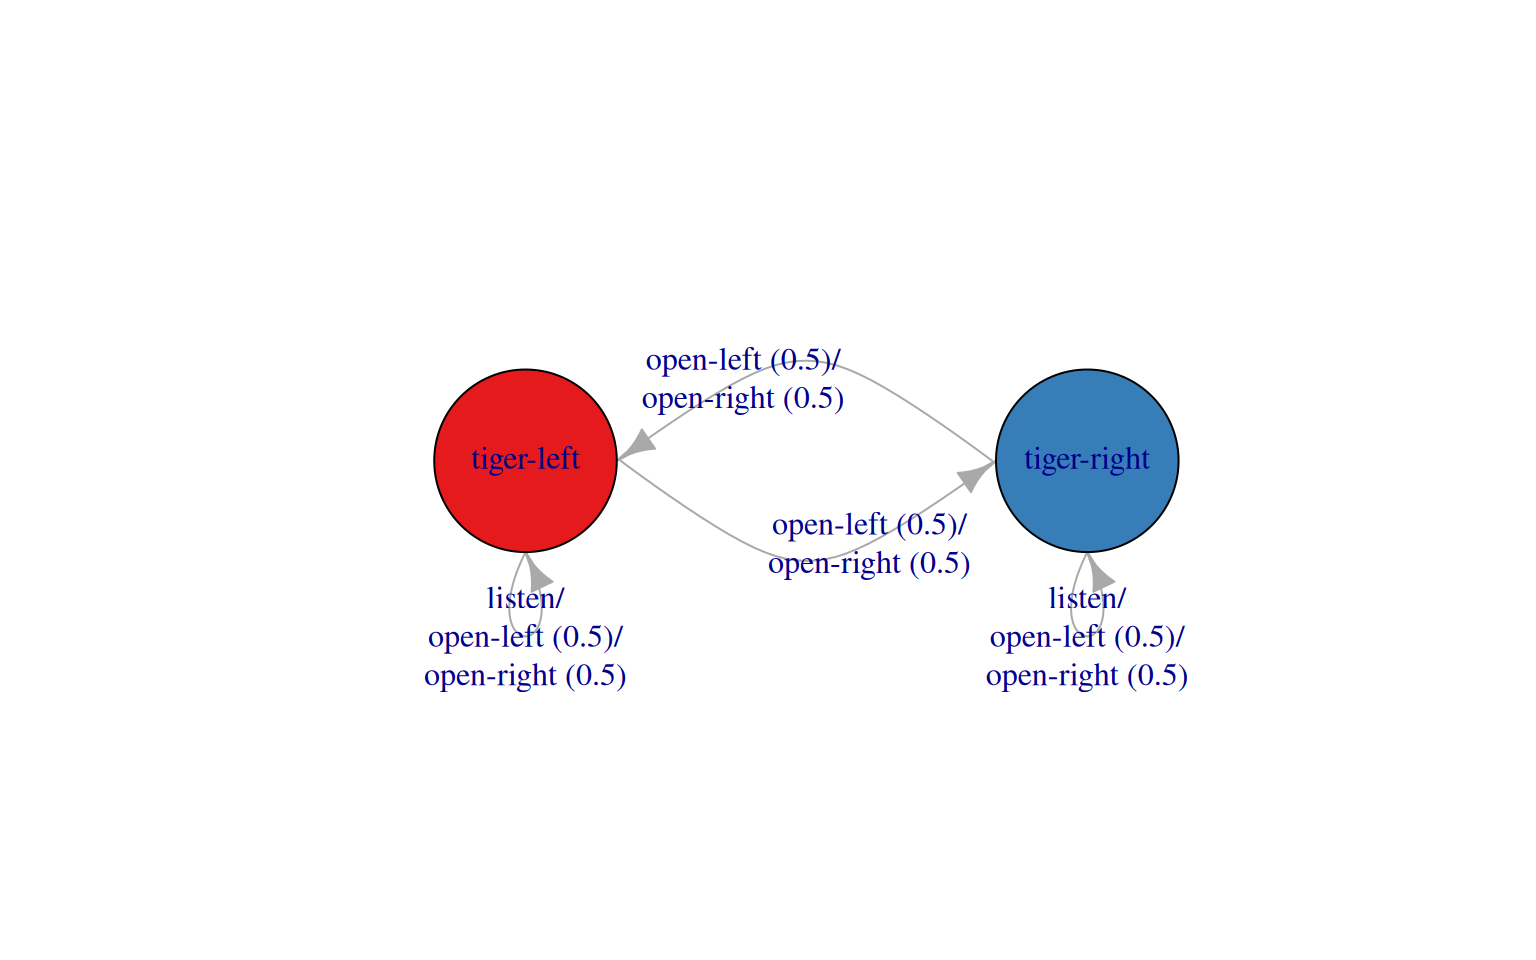
\includegraphics[width=1\linewidth]{pomdp_files/figure-latex/tiger-transition-1} \caption{Transition model of the Tiger problem.}\label{fig:tiger-transition}
\end{figure}

The vertices in Figure \ref{fig:tiger-transition} represent the states and
the edges show transitions labeled with actions and the associated transition probabilities in parentheses. Multiple parallel transitions are
collapsed into a single arrow with several labels to simplify the visualization.
The graph shows that the action \texttt{listen} stays with a probability of 1
in the same state (i.e., listening does not move the tiger). The actions \texttt{open-left} and \texttt{open-right} lead to
a reset of the problem which assigns the tiger randomly to a state. This is represented by the transitions with a
probability of .5.

For more complicated transition models, individual graphs for each action or interactive
graphs using \CRANpkg{visNetwork} can also be plotted.

\hypertarget{solving-the-tiger-problem-for-an-infinite-time-horizon}{%
\subsection{Solving the Tiger problem for an infinite time horizon}\label{solving-the-tiger-problem-for-an-infinite-time-horizon}}

To solve the problem, we use the default method (pomdp-solve's finite grid method interfaced
in package \CRANpkg{pomdpSolve})
which performs a form of point-based value iteration that can find
approximate solutions for larger problems.

\begin{verbatim}
sol <- solve_POMDP(Tiger)
sol
\end{verbatim}

\begin{verbatim}
#> POMDP, list - Tiger Problem
#>   Discount factor: 0.75
#>   Horizon: Inf epochs
#>   Size: 2 states / 3 actions / 2 obs.
#>   Start: 0.5, 0.5
#>   Normalized: TRUE
#>   Solved:
#>     Method: grid
#>     Solution converged: TRUE
#>     # of alpha vectors: 5
#>     Total expected reward: 1.933439
#> 
#>   List components: 'name', 'discount', 'horizon', 'states', 'actions',
#>     'observations', 'transition_prob', 'observation_prob', 'reward',
#>     'start', 'normalized', 'solution'
\end{verbatim}

The solver returns an object of class POMDP, which contains the solution as an
additional list component. The print function displays important information like the
used discount factor, the horizon, if the solution has converged and the total expected reward. In this case, the total expected discounted reward for following the policy starting from the initial belief is 1.933.
Note that
the optimal policy for infinite-horizon does not depend on the
initial belief.
The reward for other initial beliefs can be calculated using the
\texttt{reward()} function. For example, the expected reward for a correct
belief that the tiger starts to the left with a probability of 90\% is:

\begin{verbatim}
reward(sol, belief = c(0.9, 0.1)) 
\end{verbatim}

\begin{verbatim}
#> [1] 4.779814
\end{verbatim}

\hypertarget{inspecting-the-policy}{%
\subsection{Inspecting the Policy}\label{inspecting-the-policy}}

The policy of a solved POMDP is a set of \(\alpha\)-vectors
representing a segment of the value function and the
associated best action.

\begin{verbatim}
policy(sol)
\end{verbatim}

\begin{verbatim}
#> [[1]]
#>   tiger-left tiger-right     action
#> 1 -98.549921   11.450079  open-left
#> 2 -10.854299    6.516937     listen
#> 3   1.933439    1.933439     listen
#> 4   6.516937  -10.854299     listen
#> 5  11.450079  -98.549921 open-right
\end{verbatim}

The returned policy is a list where each element represents the \(\alpha\)-vectors
for an epoch. The policy above has only one list element since the solution
converged to a solution that is independent of the epoch.

Smaller policies that
correspond to a conditional plan
can also be represented as a graph using a custom plot function.

\begin{verbatim}
plot_policy_graph(sol)
\end{verbatim}

\begin{figure}
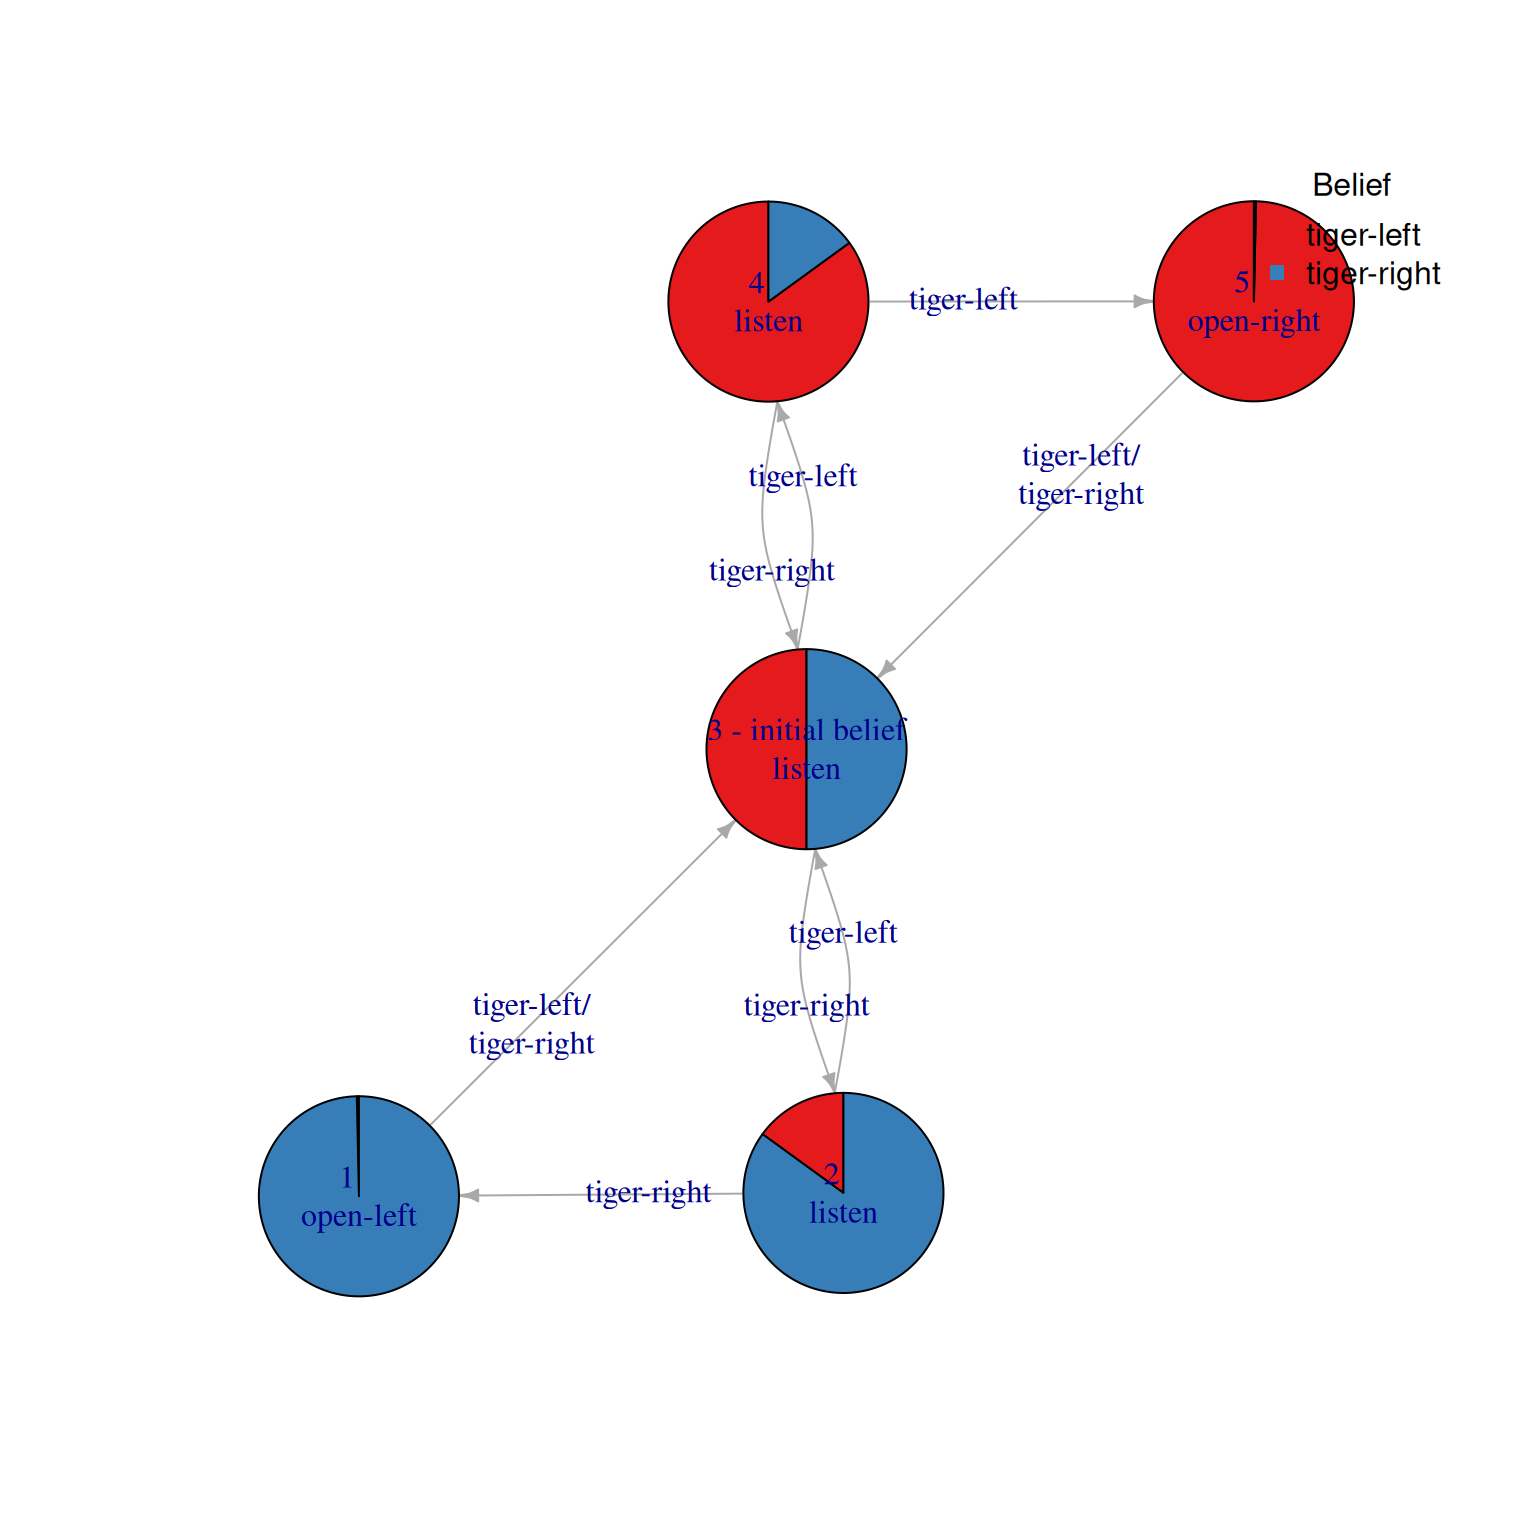
\includegraphics[width=1\linewidth]{pomdp_files/figure-latex/tiger-infinite-horizon-1} \caption{The policy graph for the converged infinite-horizon solution of the Tiger problem.}\label{fig:tiger-infinite-horizon}
\end{figure}

The function uses the \CRANpkg{igraph} package (Csardi and Nepusz 2006) to produce the layout.
Figure \ref{fig:tiger-infinite-horizon} shows the graph for the optimal policy returned
by the solver for the Tiger problem.
Each node in the policy graph represents an \(\alpha\)-vector and is labeled by the
action prescribed by the policy.
Each segment covers a part of the belief space which represents how much the agent knows about the location of
the tiger based on all previous observations.
We use a pie chart inside each node to show a representative belief point that belongs to the segment.
This makes it easier to compare the beliefs in different nodes with each other.
The representative belief points are found with the function
\texttt{estimate\_belief\_for\_nodes()} which uses the solver output and searches along policy trajectories.

It is easy to interpret smaller policy graphs. Figure \ref{fig:tiger-infinite-horizon} shows that without prior information,
the agent starts at the node marked with initial belief. In this case,
the agent believes there is a 50/50 chance that the tiger is behind
either door. The optimal action is displayed inside the state and, in this
case, is to listen. The arcs are labeled with observations. Let us
assume that the observation is tiger-left. The agent follows the
appropriate arc and ends in a node representing the new range of belief states with a higher probability of the tiger being to the left.
However, the optimal action is still to listen. If the agent again hears
the tiger on the left then it ends up in a node that has a
belief of close to 100\% that the tiger is to the left and open-right is the optimal
action. The arcs back from the nodes with the open actions to the
initial state reset the problem and let the agent start over.

Typically, small and compact policy graphs are preferable in practice because they make
the policy easier to understand for the decision maker and also easier to follow.
For large, more complicated policy graphs, representation as a graph is difficult
leading to issues with node layout and too many crossing vertices.
The package can also plot the
graph as an interactive HTML widget with movable vertices (see the manual page for \texttt{plot\_policy\_graph()})
to let the user arrange the graph manually.
Larger policy graphs can also be exported in common formats
like graphML to be displayed and analyzed in large-scale network analysis tools like Gephi (Jacomy et al. 2014).

The Tiger problem environment has only two states (tiger-left and tiger-right) with a
belief space forming a 1-simplex which is a line going from a probability of 1 that the tiger is left
to a probability of 1 that the tiger is right. Therefore, we can visualize the piecewise linear
convex value function as a simple line chart with the belief on the x-axis.

\begin{verbatim}
plot_value_function(sol, ylim = c(0,20))
\end{verbatim}

\begin{figure}
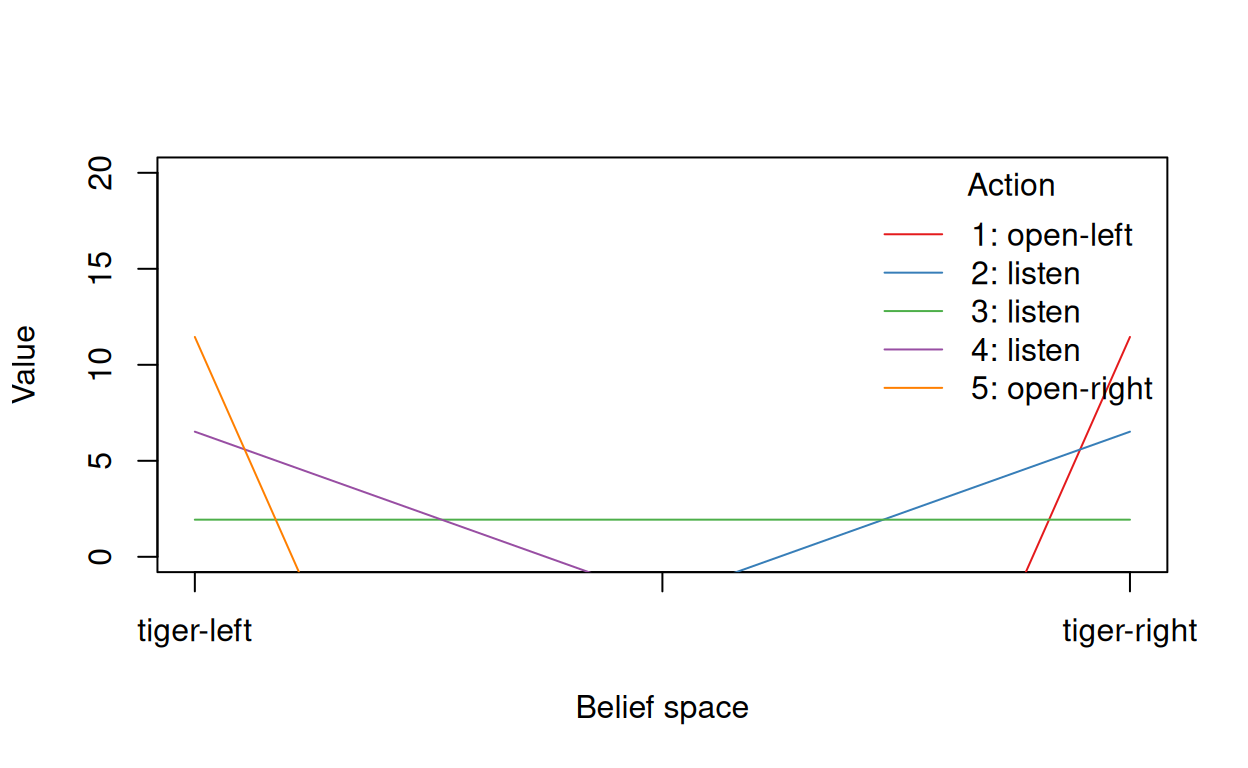
\includegraphics[width=1\linewidth]{pomdp_files/figure-latex/tiger-value-function-1} \caption{The value function for the solution of the converged Tiger problem.}\label{fig:tiger-value-function}
\end{figure}

Figure \ref{fig:tiger-value-function} shows the value function.
The x-axis represents the belief, the lines represent the nodes in the policy graph (the numbers in the legend match the numbers in the graph in Figure \ref{fig:tiger-value-function}),
and the piecewise linear value function consists of the line segments with the highest reward.
The optimal action for each segment is shown in the legend.
This visualization function is mostly provided to study small textbook examples
with two states. A more versatile function is \texttt{plot\_belief\_space()} which can produce
ternary plots for problems with three or more states by projecting the belief
space on three states.

Auxiliary functions provided in the package let the user perform many analyses. For example, we simulate
trajectories through the POMDP belief space by following the policy and estimating the distribution of the
agent's belief.

\begin{verbatim}
sim <- simulate_POMDP(sol, n = 50, horizon = 5, 
  belief = c(.5, .5), return_beliefs = TRUE)
plot_belief_space(sol, sample = sim$belief_states, ylim = c(0, 12), 
                  jitter = 5)
lines(density(sim$belief_states[, 1], bw = .01, from = 0 , to = 1)) 
axis(2); title(ylab = "Density")
\end{verbatim}

\begin{figure}
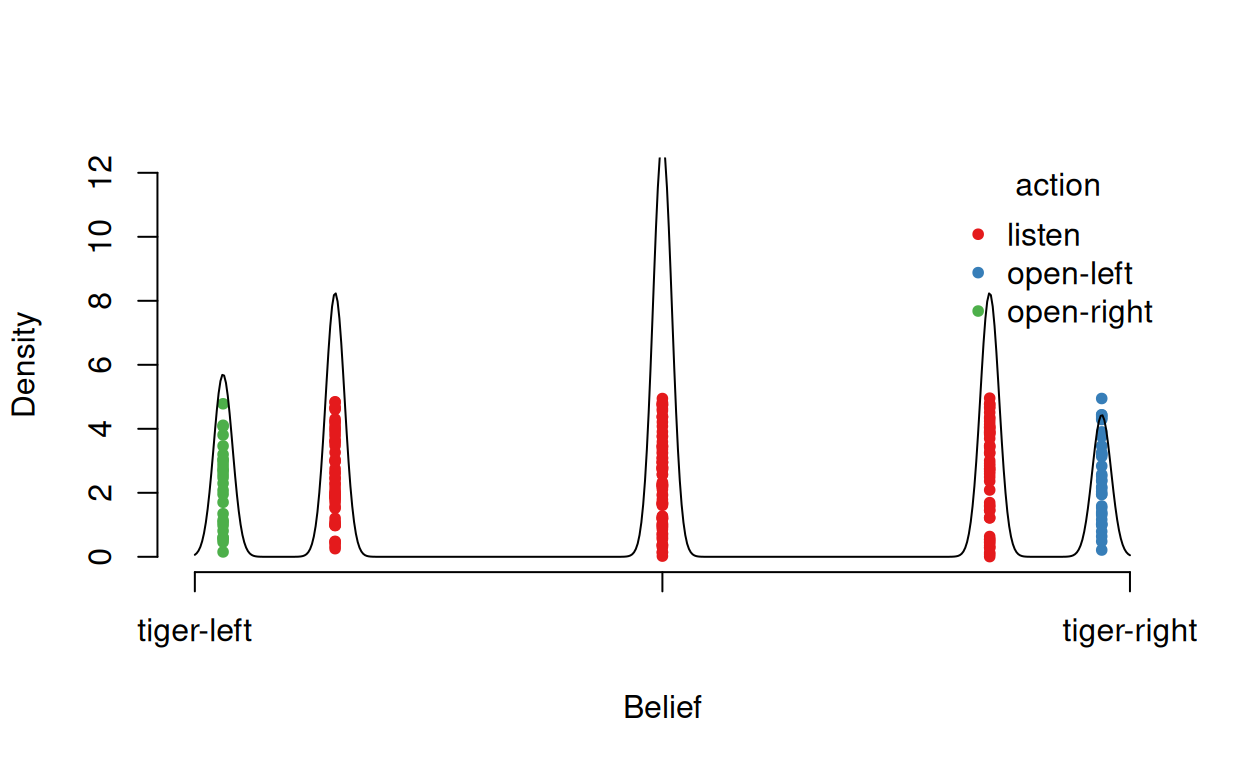
\includegraphics[width=1\linewidth]{pomdp_files/figure-latex/tiger-simulation-1} \caption{Belief states reached in 50 simulated trajectories of horizon 5.}\label{fig:tiger-simulation}
\end{figure}

Figure \ref{fig:tiger-simulation} shows the five beliefs that are
reached in the trajectories as dots and uses jitter and a density estimate to show how
much time the agent has spent in the simulation in different parts of the belief space. The color of the dots indicates the actions chosen by the policy.

\hypertarget{solving-the-tiger-problem-for-a-finite-time-horizon}{%
\subsection{Solving the Tiger problem for a finite time horizon}\label{solving-the-tiger-problem-for-a-finite-time-horizon}}

To demonstrate how to solve a POMDP problem with a finite time horizon,
we set the horizon to 4 epochs, which means that the agent starts with its initial
belief and can perform only four actions.
The grid-based method used before
finds the optimal policy, but for finite time horizon problems with negative rewards, the
value function and the calculated expected reward is only valid when the solution converges.
To avoid this issue, we use here the incremental pruning
algorithm (Zhang and Liu 1996; Cassandra, Littman, and Zhang 1997).

\begin{verbatim}
sol <- solve_POMDP(model = Tiger, horizon = 4, method = "incprune")
sol
\end{verbatim}

\begin{verbatim}
#> POMDP, list - Tiger Problem
#>   Discount factor: 0.75
#>   Horizon: 4 epochs
#>   Size: 2 states / 3 actions / 2 obs.
#>   Start: 0.5, 0.5
#>   Normalized: TRUE
#>   Solved:
#>     Method: incprune
#>     Solution converged: FALSE
#>     # of alpha vectors: 26
#>     Total expected reward: 0.483125
#> 
#>   List components: 'name', 'discount', 'horizon', 'states', 'actions',
#>     'observations', 'transition_prob', 'observation_prob', 'reward',
#>     'start', 'normalized', 'solution'
\end{verbatim}

\begin{verbatim}
policy(sol)
\end{verbatim}

\begin{verbatim}
#> [[1]]
#>   tiger-left tiger-right     action
#> 1 -99.321250   10.678750  open-left
#> 2 -11.820719    4.640094     listen
#> 3  -2.734955    2.600990     listen
#> 4  -1.137420    1.595135     listen
#> 5   0.483125    0.483125     listen
#> 6   1.595135   -1.137420     listen
#> 7   2.600990   -2.734955     listen
#> 8   4.640094  -11.820719     listen
#> 9  10.678750  -99.321250 open-right
#> 
#> [[2]]
#>    tiger-left tiger-right     action
#> 1 -101.312500    8.687500  open-left
#> 2  -20.550156    5.488906     listen
#> 3  -13.450000    4.700000     listen
#> 4   -3.565469    2.157969     listen
#> 5    0.905000    0.905000     listen
#> 6    2.157969   -3.565469     listen
#> 7    4.700000  -13.450000     listen
#> 8    5.488906  -20.550156     listen
#> 9    8.687500 -101.312500 open-right
#> 
#> [[3]]
#>   tiger-left tiger-right     action
#> 1  -100.7500      9.2500  open-left
#> 2   -12.8875      5.2625     listen
#> 3    -1.7500     -1.7500     listen
#> 4     5.2625    -12.8875     listen
#> 5     9.2500   -100.7500 open-right
#> 
#> [[4]]
#>   tiger-left tiger-right     action
#> 1       -100          10  open-left
#> 2         -1          -1     listen
#> 3         10        -100 open-right
\end{verbatim}

The policy has four elements, one for each epoch. Is easier to understand the
policy by visualizing it as a graph.

\begin{verbatim}
plot_policy_graph(sol)
\end{verbatim}

\begin{figure}
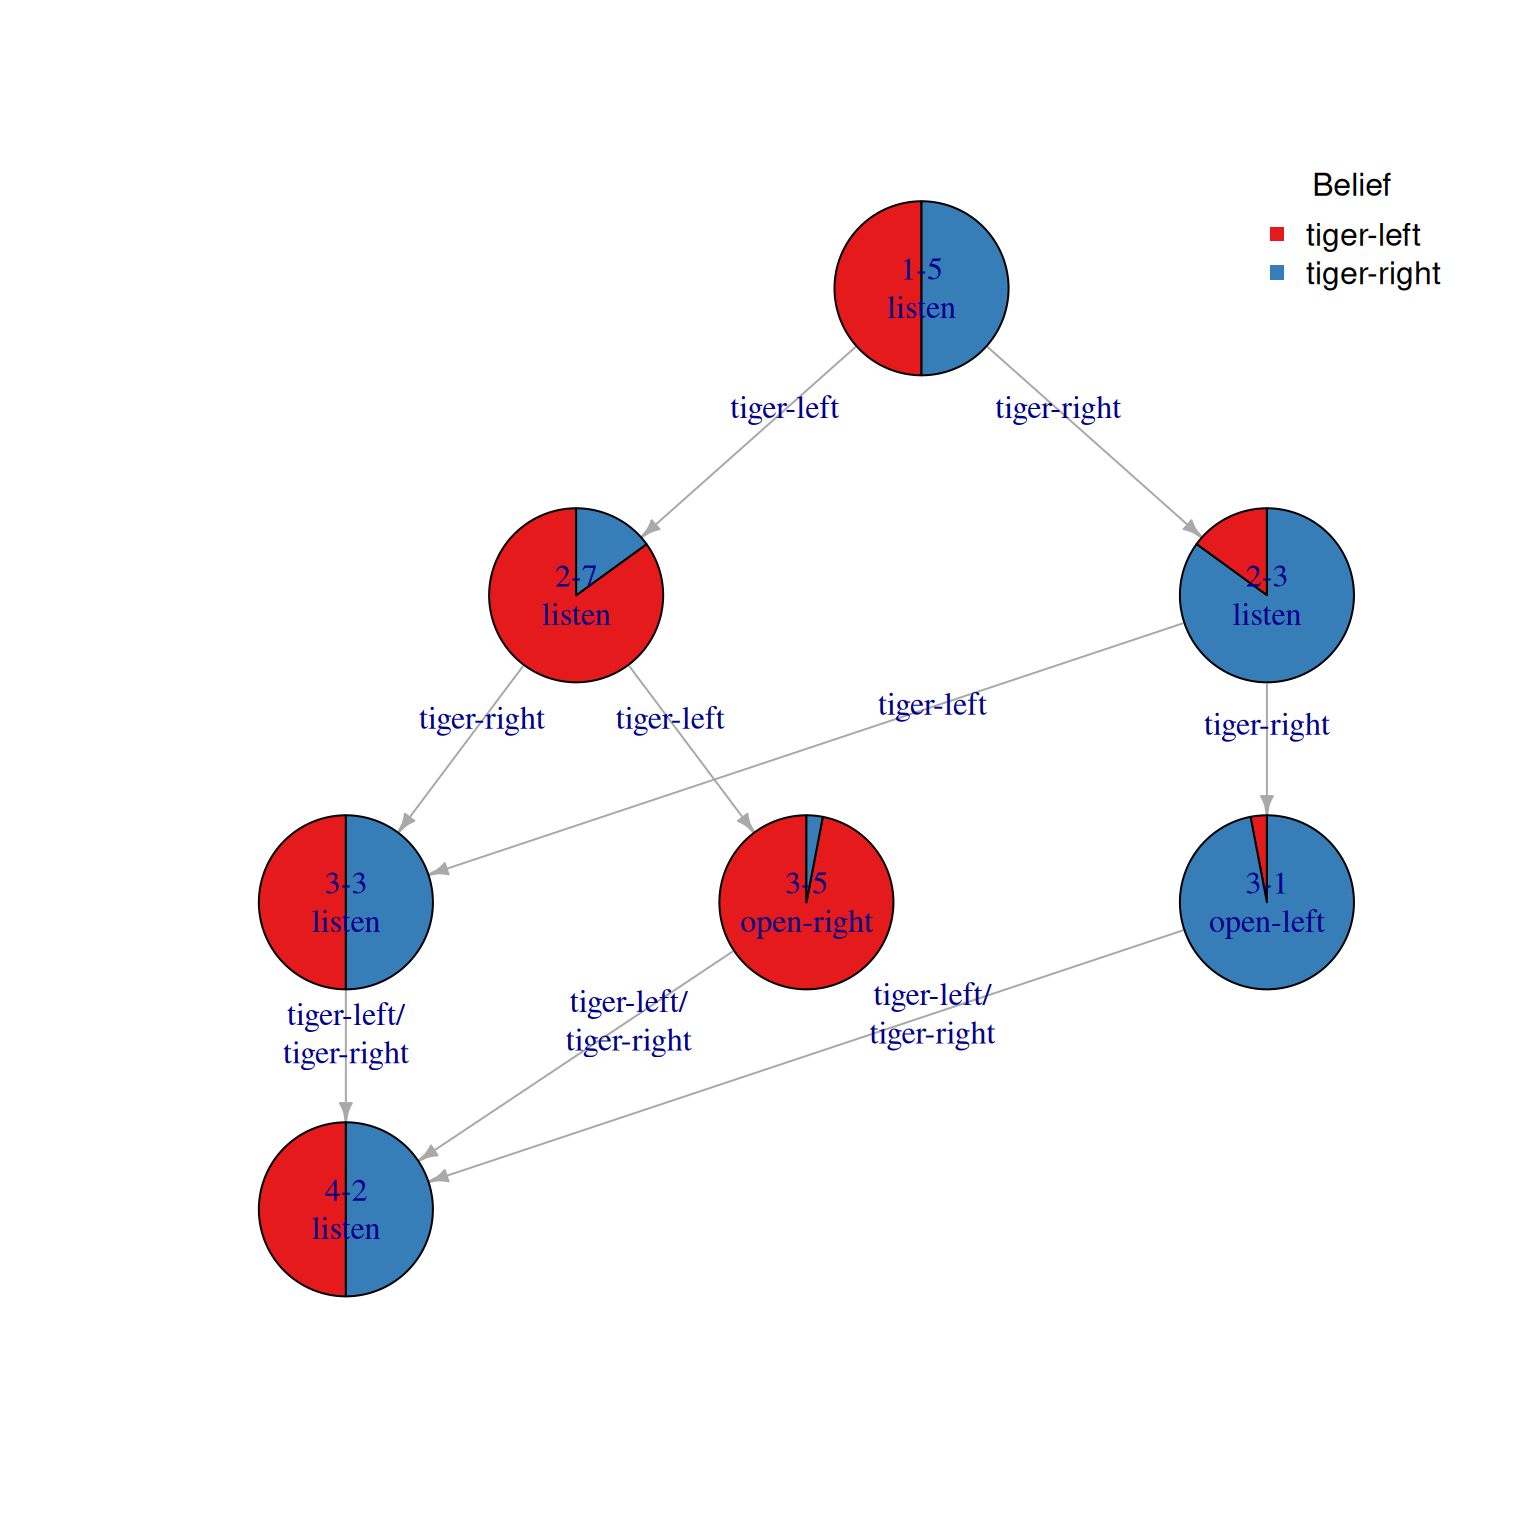
\includegraphics[width=1\linewidth]{pomdp_files/figure-latex/tiger-finite-horizon-1} \caption{Policy tree for the Tiger problem solved with a horizon of 4 and a uniform initial belief.}\label{fig:tiger-finite-horizon}
\end{figure}

The resulting policy graph is shown in Figure \ref{fig:tiger-finite-horizon}
as a tree with four levels, one for each time epoch. The plot function automatically
uses a tree layout and adds the epoch as the first number to the node labels. By default,
it also simplifies the representation by hiding belief states which cannot be reached
form the start belief and, therefore, there are more entries in the policy above
than there are nodes in the graph.
The root node of the tree represents the initial belief
used in the model. The model starts with a uniform initial belief represented by the evenly split pie chart.
The policy shows that
the optimal strategy is
to listen and open a door only if we hear the tiger behind the same door twice.
Interestingly, it is optimal never to open a door in
the last epoch. The reason is that we cannot reach a sufficiently high belief of the tiger being behind a single door.
The expected reward of this policy starting at a uniform initial belief is
0.483.

Policy trees for finite-horizon problems are dependent on the agent's
initial belief. To show this, we produce a new policy tree
for an initial belief of 99\% that the tiger is to the left by overwriting the initial belief in the model definition.

\begin{verbatim}
sol <- solve_POMDP(model = Tiger, horizon = 4, 
  initial_belief = c(.99, .01), method = "incprune")
reward(sol, belief = c(.99, .01))
\end{verbatim}

\begin{verbatim}
#> [1] 9.57875
\end{verbatim}

\begin{verbatim}
plot_policy_graph(sol, belief = c(.99, .01))
\end{verbatim}

\begin{figure}
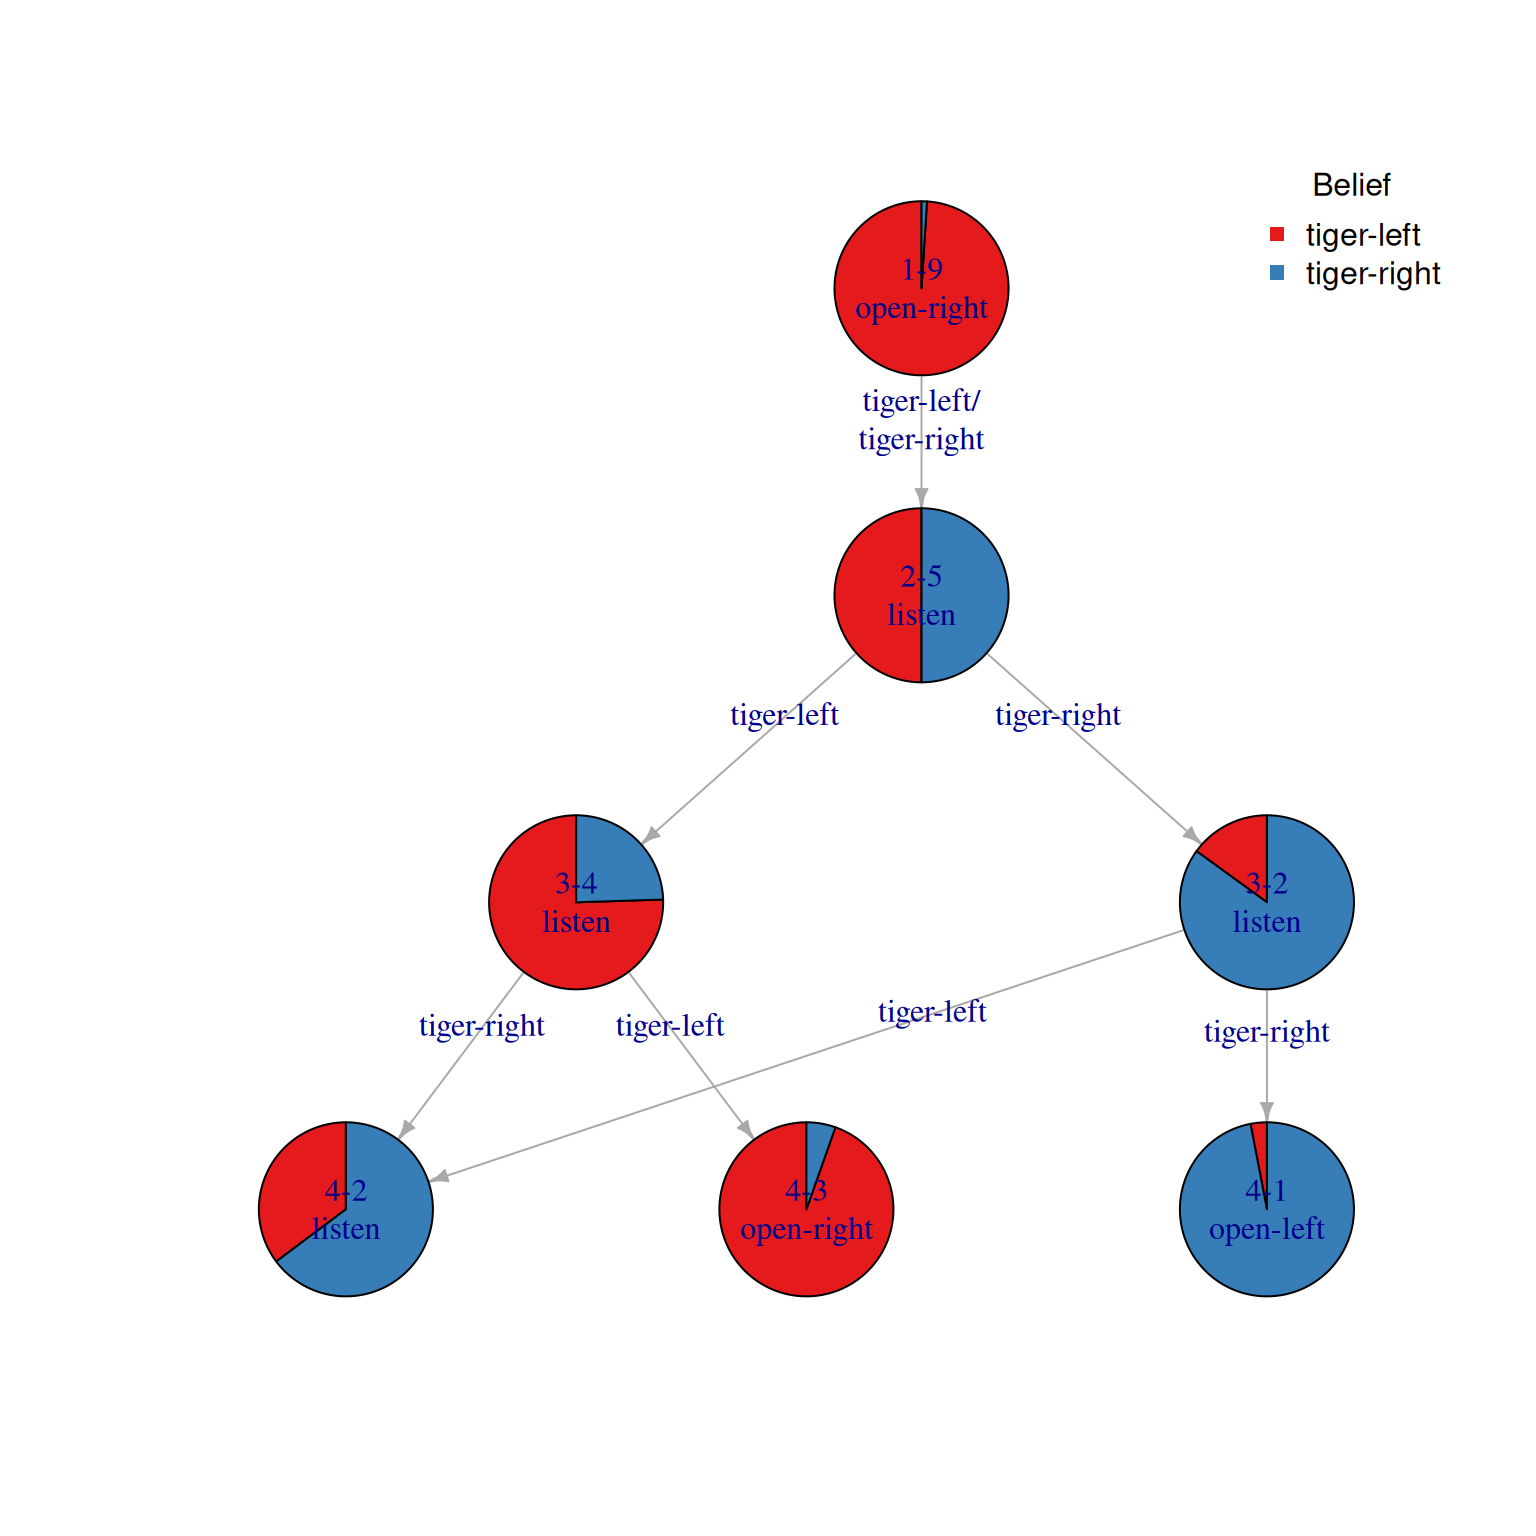
\includegraphics[width=1\linewidth]{pomdp_files/figure-latex/tiger-finite-horizon-99-1} \caption{Policy tree for the Tiger problem solved with a horizon of 4 and an initial belief of 99 percent that the tiger is to the left.}\label{fig:tiger-finite-horizon-99}
\end{figure}

The resulting policy graph with an initial belief indicating that we are very sure that the tiger
is to the left is shown in Figure \ref{fig:tiger-finite-horizon-99}. The graph
indicates that it is optimal to open the right door right away and then wait if we hear the tiger twice in the same location before we open the other door.
Under the strong belief, the agent also expects a much higher reward of
9.579 for the optimal policy.

\hypertarget{summary}{%
\section{Summary}\label{summary}}

Partially observable Markov decision processes are an important modeling technique useful
for many applications.
Easily accessible software to solve POMDP problems is crucial to support applied research and instruction in fields including artificial intelligence and operations research. Most existing libraries need advanced technical expertise to install and offer minimal support to analyze the results. The \CRANpkg{pomdp} package fills this gap by providing an easily accessible platform to perform experiments and analyze POMDP problems and the resulting policies.

This paper used a minimalist toy example to show the functionality of the package in
a concise way.
Studying and visualizing complicated policies with hundreds or thousands of belief states
is an important topic that has received less attention than improving solver algorithms.
R provides a wide range of tools to compare, analyze, and cluster belief states. We plan
to investigate the use of these techniques to support
explainability of more complicated policies and will implement corresponding functions in
future releases of the package \CRANpkg{pomdp}.

\hypertarget{acknowledgments}{%
\section{Acknowledgments}\label{acknowledgments}}

Farzad Kamalzadeh participated in the development of an early version of the pomdp package
and used it for several applications.
He was supported by a Graduate Fellowship and a Niemi Center Fellowship, both at SMU.
His and Michael Hahsler's work was also supported in part by
the National Institute of Standards and Technology (NIST) under grant number 60NANB17D180.

The authors would also like to thank Carl Boettiger for maintaining the package
\CRANpkg{sarsop} and the anonymous reviewers for their valuable insights.

\hypertarget{references}{%
\section*{References}\label{references}}
\addcontentsline{toc}{section}{References}

\hypertarget{refs}{}
\begin{CSLReferences}{1}{0}
\leavevmode\vadjust pre{\hypertarget{ref-Almende2022}{}}%
Almende B.V. and Contributors, and Benoit Thieurmel. 2022. \emph{visNetwork: Network Visualization Using 'Vis.js' Library}. \url{https://CRAN.R-project.org/package=visNetwork}.

\leavevmode\vadjust pre{\hypertarget{ref-APPL2022}{}}%
APPL Team. 2022. {``{APPL}: {A}pproximate {POMDP} Planning Toolkit.''} \url{https://bigbird.comp.nus.edu.sg/pmwiki/farm/appl/}.

\leavevmode\vadjust pre{\hypertarget{ref-Astrom1965}{}}%
Åström, K. J. 1965. {``Optimal Control of {M}arkov Processes with Incomplete State Information.''} \emph{Journal of Mathematical Analysis and Applications} 10 (1): 174--205.

\leavevmode\vadjust pre{\hypertarget{ref-Bates2022}{}}%
Bates, Douglas, Martin Maechler, and Mikael Jagan. 2022. \emph{Matrix: Sparse and Dense Matrix Classes and Methods}. \url{https://CRAN.R-project.org/package=Matrix}.

\leavevmode\vadjust pre{\hypertarget{ref-Bottiger2021}{}}%
Boettiger, Carl, Jeroen Ooms, and Milad Memarzadeh. 2021. \emph{Sarsop: {A}pproximate {POMDP} Planning Software}. \url{https://CRAN.R-project.org/package=sarsop}.

\leavevmode\vadjust pre{\hypertarget{ref-Cassandra1998b}{}}%
Cassandra, Anthony R. 1998a. {``A Survey of {POMDP} Applications.''} MCC-INSL-111-98. Microelectronics; Computer Technology Corporation (MCC).

\leavevmode\vadjust pre{\hypertarget{ref-Cassandra1998}{}}%
---------. 1998b. {``Exact and Approximate Algorithms for Partially Observable Markov Decision Processes.''} PhD thesis, Providence, RI, USA: Brown University.

\leavevmode\vadjust pre{\hypertarget{ref-Cassandra2015}{}}%
---------. 2015. {``The {POMDP} Page.''} \url{https://www.pomdp.org}.

\leavevmode\vadjust pre{\hypertarget{ref-Cassandra1994}{}}%
Cassandra, Anthony R., Leslie Pack Kaelbling, and Michael L. Littman. 1994. {``Acting Optimally in Partially Observable Stochastic Domains.''} In \emph{Proceedings of the Twelfth National Conference on Artificial Intelligence}. Seattle, WA.

\leavevmode\vadjust pre{\hypertarget{ref-Cassandra1997}{}}%
Cassandra, Anthony R., Michael L. Littman, and Nevin Lianwen Zhang. 1997. {``Incremental Pruning: {A} Simple, Fast, Exact Method for Partially Observable {M}arkov Decision Processes.''} In \emph{UAI'97: Proceedings of the Thirteenth Conference on Uncertainty in Artificial Intelligence}, 54-\/-61.

\leavevmode\vadjust pre{\hypertarget{ref-igraph2006}{}}%
Csardi, Gabor, and Tamas Nepusz. 2006. {``The Igraph Software Package for Complex Network Research.''} \emph{InterJournal} Complex Systems: 1695. \url{https://igraph.org}.

\leavevmode\vadjust pre{\hypertarget{ref-Eddelbuettel2013}{}}%
Eddelbuettel, Dirk. 2013. \emph{Seamless {R} and {C++} Integration with {Rcpp}}. New York: Springer. \url{https://doi.org/10.1007/978-1-4614-6868-4}.

\leavevmode\vadjust pre{\hypertarget{ref-Hahsler2022}{}}%
Hahsler, Michael. 2023. \emph{Pomdp: Infrastructure for Partially Observable Markov Decision Processes (POMDP)}. \url{https://github.com/mhahsler/pomdp}.

\leavevmode\vadjust pre{\hypertarget{ref-Hahsler2022b}{}}%
Hahsler, Michael, and Anthony R. Cassandra. 2022. \emph{pomdpSolve: Interface to 'Pomdp-Solve' for Partially Observable Markov Decision Processes}. \url{https://github.com/mhahsler/pomdpSolve}.

\leavevmode\vadjust pre{\hypertarget{ref-Hauskrecht2000}{}}%
Hauskrecht, Milos. 2000. {``Value-Function Approximations for {POMDPs}.''} \emph{Journal Of Artificial Intelligence Research} 13: 33--94. https://doi.org/\url{https://doi.org/10.1613/jair.678}.

\leavevmode\vadjust pre{\hypertarget{ref-Jacomy2014}{}}%
Jacomy, Mathieu, Tommaso Venturini, Sebastien Heymann, and Mathieu Bastian. 2014. {``ForceAtlas2, a Continuous Graph Layout Algorithm for Handy Network Visualization Designed for the {G}ephi Software.''} \emph{PLOS ONE} 9 (6): 1--12. \url{https://doi.org/10.1371/journal.pone.0098679}.

\leavevmode\vadjust pre{\hypertarget{ref-juliapomdp2022}{}}%
JuliaPOMDP Team. 2022. {``{JuliaPOMDP:} {POMDP} Packages for {Julia}.''} \url{https://github.com/JuliaPOMDP}.

\leavevmode\vadjust pre{\hypertarget{ref-Kaelbling1998}{}}%
Kaelbling, Leslie Pack, Michael L. Littman, and Anthony R. Cassandra. 1998. {``Planning and Acting in Partially Observable Stochastic Domains.''} \emph{Artificial Intelligence} 101 (1): 99--134. \url{https://doi.org/10.1016/S0004-3702(98)00023-X}.

\leavevmode\vadjust pre{\hypertarget{ref-hahsler:Kamalzadeh:2021}{}}%
Kamalzadeh, Farzad, Vishal Ahuja, Michael Hahsler, and Michael E. Bowen. 2021. {``An Analytics-Driven Approach for Optimal Individualized Diabetes Screening.''} \emph{Production and Operations Management} 30 (9): 3161--91. \url{https://doi.org/10.1111/poms.13422}.

\leavevmode\vadjust pre{\hypertarget{ref-Kurniawati2008}{}}%
Kurniawati, Hanna, David Hsu, and Wee Sun Lee. 2008. {``{SARSOP:} {E}fficient Point-Based POMDP Planning by Approximating Optimally Reachable Belief Spaces.''} In \emph{In Proc. Robotics: Science and Systems}.

\leavevmode\vadjust pre{\hypertarget{ref-Littman1995}{}}%
Littman, Michael L., Anthony R. Cassandra, and Leslie Pack Kaelbling. 1995. {``Learning Policies for Partially Observable Environments: {S}caling Up.''} In \emph{Proceedings of the Twelfth International Conference on International Conference on Machine Learning}, 362--70. ICML'95. San Francisco, CA, USA: Morgan Kaufmann Publishers Inc.

\leavevmode\vadjust pre{\hypertarget{ref-Microsoft2022}{}}%
Microsoft, and Steve Weston. 2022. \emph{Foreach: Provides Foreach Looping Construct}. \url{https://CRAN.R-project.org/package=foreach}.

\leavevmode\vadjust pre{\hypertarget{ref-pypomdp2013}{}}%
Migge, Bastian, and Oliver Stollmann. 2013. {``{pyPOMDP:} {POMDP} Implementation in {Python}.''} \url{https://bitbucket.org/bami/pypomdp/src/master/}.

\leavevmode\vadjust pre{\hypertarget{ref-Monahan1982}{}}%
Monahan, G. E. 1982. {``A Survey of Partially Observable {M}arkov Decision Processes: {T}heory, Models, and Algorithms.''} \emph{Management Science} 28 (1): 1--16.

\leavevmode\vadjust pre{\hypertarget{ref-Mundhenk2000}{}}%
Mundhenk, Martin. 2000. {``The Complexity of Optimal Small Policies.''} \emph{Math. Oper. Res.} 25 (1): 118--29.

\leavevmode\vadjust pre{\hypertarget{ref-Pineau2003}{}}%
Pineau, Joelle, Geoff Gordon, and Sebastian Thrun. 2003. {``Point-Based Value Iteration: {A}n Anytime Algorithm for {POMDPs}.''} In \emph{Proceedings of the 18th International Joint Conference on Artificial Intelligence}, 1025--30. IJCAI'03. San Francisco, CA, USA: Morgan Kaufmann Publishers Inc.

\leavevmode\vadjust pre{\hypertarget{ref-Proellochs2020}{}}%
Proellochs, Nicolas, and Stefan Feuerriegel. 2020. \emph{ReinforcementLearning: {M}odel-Free Reinforcement Learning}. \url{https://CRAN.R-project.org/package=ReinforcementLearning}.

\leavevmode\vadjust pre{\hypertarget{ref-Puterman1994}{}}%
Puterman, Martin L. 1994. {``Markov Decision Processes: {D}iscrete Stochastic Dynamic Programming.''} In \emph{Wiley Series in Probability and Statistics}.

\leavevmode\vadjust pre{\hypertarget{ref-Smallwood1973}{}}%
Smallwood, R. D., and E. J. Sondik. 1973. {``The Optimal Control of Partially Observable {M}arkov Decision Processes over a Finite Horizon.''} \emph{Operations Research} 21 (5): 1071--88.

\leavevmode\vadjust pre{\hypertarget{ref-ZMDP2009}{}}%
Smith, T. 2009. {``{ZMDP}: {S}oftware for {POMDP} and {MDP} Planning.''} \url{https://github.com/trey0/zmdp}.

\leavevmode\vadjust pre{\hypertarget{ref-Sondik1971}{}}%
Sondik, E. J. 1971. {``The Optimal Control of Partially Observable {M}arkov Decision Processes.''} PhD thesis, Stanford, California.

\leavevmode\vadjust pre{\hypertarget{ref-Sutton1998}{}}%
Sutton, Richard S., and Andrew G. Barto. 2018. \emph{Reinforcement Learning: {A}n Introduction}. Second. The MIT Press.

\leavevmode\vadjust pre{\hypertarget{ref-Wickham2016}{}}%
Wickham, Hadley. 2016. \emph{Ggplot2: Elegant Graphics for Data Analysis}. Springer-Verlag New York. \url{https://ggplot2.tidyverse.org}.

\leavevmode\vadjust pre{\hypertarget{ref-Zhang1996}{}}%
Zhang, Nevin L., and Wenju Liu. 1996. {``Planning in Stochastic Domains: {P}roblem Characteristics and Approximation.''} HKUST-CS96-31. Hong Kong University.

\end{CSLReferences}

\bibliography{pomdp.bib}

\address{%
Michael Hahsler\\
Southern Methodist University\\%
Department of Computer Science\\ Dallas, TX, USA\\
%
\url{https://michael.hahsler.net}\\%
\textit{ORCiD: \href{https://orcid.org/0000-0003-2716-1405}{0000-0003-2716-1405}}\\%
\href{mailto:mhahsler@lyle.smu.edu}{\nolinkurl{mhahsler@lyle.smu.edu}}%
}

\address{%
Anthony R. Cassandra\\
POMDP, Inc\\%
Austin, TX, USA\\
%
\url{https://tonycassandra.com}\\%
%
\href{mailto:tony.cassandra@igmail.com}{\nolinkurl{tony.cassandra@igmail.com}}%
}
